\clearpage

\begin{tcolorbox}	
\begin{tabular}{p{2.75cm} p{0.2cm} p{10.5cm}} 	
\textbf{Student Name}  &:& Tiago Esteves\\
\textbf{Starting Date} &:& October 03, 2017\\
\textbf{Goal}          &:& Implement the dimensioning of optical networks in the translucent transport mode.
\end{tabular}
\end{tcolorbox}

\section{Translucent with 1+1 Protection}

In this case study we focus on the translucent case with 1 + 1 protection. Translucent transport mode is a combination of previous transport modes. Thus, for the same physical topology, there are several logical topologies.
In translucent transport mode a multi-hop cleaning scheme is employed, so different source and destination nodes can share the same light path until they reach some intermediate node common to both.
Thus, on all network nodes, light paths that carry local or client traffic that need to be switched to a different light path are sent to the electrical domain, while the light paths of traffic are maintained in the optical domain.

\subsection{Physical Network Topology}

\subsubsection{Reference Network}
In the figure below we ca see that our reference network consists of 6 nodes and 8 Bidirectional links.
The average length of the links was chosen so that the following calculations are more simplistic, for this was created a matrix of distances between the respective nodes.
Finally, ODU's matrices were also created to be able to determine the total traffic used in each scenario.

\begin{figure}[h!]
\centering
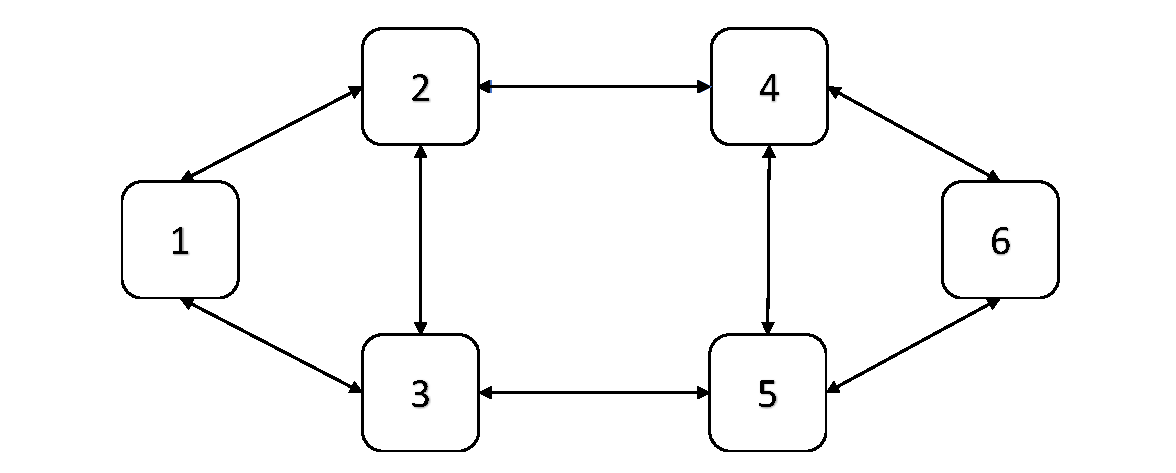
\includegraphics[width=\textwidth]{RedeTeste}
\caption{Physical Topology of the Reference Network.}
\end{figure}

The distance matrix is the same for the two scenarios but the ODU's matrices are not.
In this way only the matrices for the case of low traffic are elucidated, being that in the case of a high traffic it is only necessary to multiply these matrices by the value 10.

\[
Dist=
  \begin{bmatrix}
    0 & 500 & 500 & 0 & 0 & 0 \\
    500 & 0 & 400 & 500 & 0 & 0 \\
    500 & 400 & 0 & 0 & 500 & 0 \\
    0 & 500 & 0 & 0 & 600 & 450 \\
    0 & 0 & 500 & 600 & 0 & 550 \\
    0 & 0 & 0 & 450 & 550 & 0
  \end{bmatrix}
\]

\[
ODU0=
  \begin{bmatrix}
    0 & 5 & 1 & 3 & 1 & 3 \\
    5 & 0 & 0 & 1 & 5 & 0 \\
    1 & 0 & 0 & 1 & 4 & 1 \\
    3 & 1 & 1 & 0 & 1 & 0 \\
    1 & 5 & 4 & 1 & 0 & 3 \\
    3 & 0 & 1 & 1 & 3 & 0
  \end{bmatrix}
\quad ODU1=
  \begin{bmatrix}
    0 & 2 & 4 & 2 & 0 & 5 \\
    2 & 0 & 0 & 3 & 1 & 1 \\
    4 & 0 & 0 & 1 & 1 & 0 \\
    3 & 3 & 1 & 0 & 1 & 3 \\
    0 & 1 & 1 & 1 & 0 & 1 \\
    5 & 1 & 0 & 3 & 1 & 0
  \end{bmatrix}
\quad ODU2=
  \begin{bmatrix}
    0 & 1 & 1 & 1 & 0 & 0 \\
    1 & 0 & 0 & 0 & 1 & 0 \\
    1 & 0 & 0 & 1 & 1 & 0 \\
    1 & 0 & 1 & 0 & 1 & 0 \\
    0 & 1 & 1 & 1 & 0 & 1 \\
    0 & 0 & 0 & 0 & 1 & 0
  \end{bmatrix}
\]
\[
ODU3=
  \begin{bmatrix}
    0 & 0 & 0 & 0 & 0 & 0 \\
    0 & 0 & 1 & 0 & 0 & 1 \\
    0 & 1 & 0 & 0 & 1 & 0 \\
    0 & 0 & 0 & 0 & 0 & 0 \\
    0 & 0 & 1 & 0 & 0 & 0 \\
    0 & 1 & 0 & 0 & 0 & 0
  \end{bmatrix}
\qquad ODU4=
  \begin{bmatrix}
    0 & 0 & 0 & 0 & 0 & 0 \\
    0 & 0 & 0 & 0 & 0 & 1 \\
    0 & 0 & 0 & 0 & 0 & 0 \\
    0 & 0 & 0 & 0 & 0 & 0 \\
    0 & 0 & 0 & 0 & 0 & 1 \\
    0 & 1 & 0 & 0 & 1 & 0
  \end{bmatrix}
\]

\vspace{17pt}

The values indicated in the distance matrix, referred to below, are expressed in kilometers (Km) and as it couldn't be otherwise, this matrix is symmetric.
In relation to the traffic matrices each ODU, referred previously, has its respective value being that the ODU0 corresponds to 1.25 Gbits/s, ODU1 to 2.5 Gbits/s, ODU2 to 10 Gbits/s, ODU3 to 40 Gbits/s and finally the ODU4 corresponds to 100 Gbits/s.
As we can see these matrices are bidirectional because they are symmetric matrices and as such the traffic sent in one direction must be the same traffic sent in the opposite direction. \\

Through these ODU's we can calculate total network traffic for the low traffic scenario:\\

$T_1^0$ = 60x1.25 = 75 Gbits/s \qquad
$T_1^1$ = 50x2.5 = 125 Gbits/s \qquad
$T_1^2$ = 16x10 = 160 Gbits/s \\

$T_1^3$ = 6x40 = 240 Gbits/s \quad
$T_1^4$ = 4x100 = 400 Gbits/s \\

$T_{1}$ = 75 + 125 + 160 + 240 + 400 = 1000 Gbits/s \qquad
$T$ = 1000/2 = 0.5 Tbits/s\\

Where the variable $T_1^x$ represents the unidirectional traffic of the ODUx, for example, $T_1^2$ represents the unidirectional traffic of the ODU2 and $T_1^3$ represents the unidirectional traffic of the ODU3. The variable $T_{1}$ represents the total of unidirectional traffic that is injected into the network and finally the variable $T$ represents the total of bidirectional traffic.\\

We can thus conclude that the total traffic for the two scenarios is as follows:
\begin{itemize}
  \item Low Traffic: \textbf{0.5 TBits/s}
  \item High Traffic: \textbf{5 TBits/s}
\end{itemize}

Finally for this project has to take into consideration the table \ref{table:5} because in it we can see the values of the variables associated with this network.
\begin{table}[h!]
\centering
\begin{tabular}{|| c | c | c||}
 \hline
 Constant & Description & Value \\
 \hline\hline
 N & Number of nodes & 6 \\
 L & Number of bidirectional links & 8 \\
 <$\delta$> & Node out-degree & 2.667 \\
 <len> & Mean link length (km) & 500 \\
 <h> & Mean number of hops for working paths & 1.533 \\
 <h'> & Mean number of hops for backup paths & 2.467 \\
 \hline
\end{tabular}
\caption{Table of reference network values}
\label{table:5}
\end{table}

\subsubsection{Realistic Network}
The real network chosen for this work is the EON (European Optical Network).

\begin{figure}[h!]
\centering
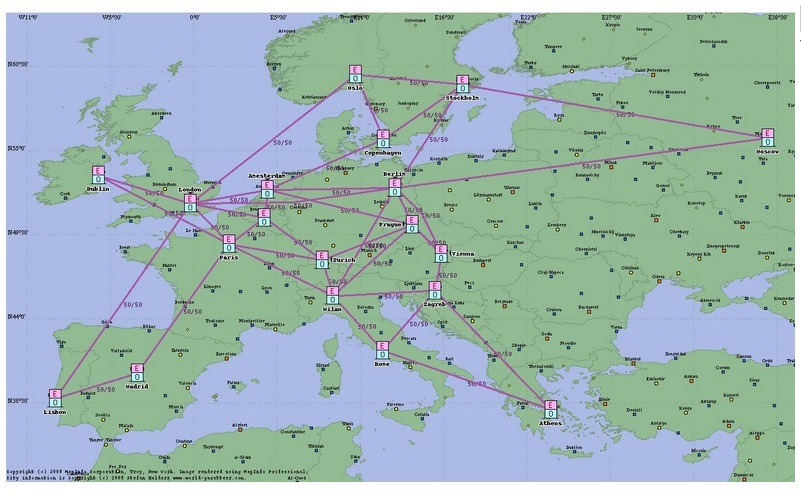
\includegraphics[width=\textwidth]{EON_Rede_Realista}
\caption{Physical Topology of the Realistic Network.}
\end{figure}

Through the previous figure we can see how nodes are organized geographically and the distance matrix created on the next page is constructed based on real distances between them.
For a better understanding of the distances matrix the table \ref{city_nodes3} was created to assign to each city a number of a node in the network.

\begin{table}[h!]
\centering
\begin{tabular}{|| c | c ||}
 \hline
 City & Node \\
 \hline\hline
 Oslo & 1 \\
 Stockholm & 2 \\
 Moscow & 3 \\
 Copenhagen & 4 \\
 Berlin & 5 \\
 Prague & 6 \\
 Vienna & 7 \\
 Zagreb & 8 \\
 Athens & 9 \\
 Rome & 10 \\
 Milan & 11 \\
 Zurich & 12 \\
 Brussels & 13 \\
 Amesterdan & 14 \\
 London & 15 \\
 Dublin & 16 \\
 Paris & 17 \\
 Madrid & 18 \\
 Lisbon & 19 \\
 \hline
\end{tabular}
\caption{Table of city and respective node}
\label{city_nodes3}
\end{table}

In this real case we have once again to take into consideration the table \ref{table:6} because it is through it that we can see the values of the variables associated with this network.

\begin{table}[h!]
\centering
\begin{tabular}{|| c | c | c||}
 \hline
 Constant & Description & Value \\
 \hline\hline
 N & Number of nodes & 19 \\
 L & Number of bidirectional links & 37 \\
 <$\delta$> & Node out-degree & 3.89 \\
 <len> & Mean link length (km) & 753.76 \\
 <h> & Mean number of hops for working paths & 2.3 \\
 <h'> & Mean number of hops for backup paths & 3.2 \\
 \hline
\end{tabular}
\caption{Table of realistic network values}
\label{table:6}
\end{table}

The values indicated in the distance matrix, referred to below, are expressed in kilometers (Km).
For this network we must also create matrices of ODU's to determine the total traffic used in each scenario but in this case only the matrices for low traffic are elucidated.


\begin{sidewaysfigure}

\[
Dist=
  \begin{pmatrix}
    0 & 417 & 0 & 484 & 0 & 0 & 0 & 0 & 0 & 0 & 0 & 0 & 0 & 0 & 1155 & 0 & 0 & 0 & 0 \\
    417 & 0 & 1228 & 523 & 811 & 0 & 0 & 0 & 0 & 0 & 0 & 0 & 0 & 0 & 0 & 0 & 0 & 0 & 0 \\
    0 & 1228 & 0 & 0 & 1611 & 0 & 0 & 0 & 0 & 0 & 0 & 0 & 0 & 0 & 0 & 0 & 0 & 0 & 0 \\
    484 & 523 & 0 & 0 & 0 & 0 & 0 & 0 & 0 & 0 & 0 & 0 & 0 & 622 & 0 & 0 & 0 & 0 & 0 \\
    0 & 811 & 1611 & 0 & 0 & 281 & 524 & 0 & 0 & 0 & 843 & 0 & 0 & 577 & 933 & 0 & 0 & 0 & 0 \\
    0 & 0 & 0 & 0 & 281 & 0 & 251 & 0 & 0 & 0 & 646 & 527 & 0 & 712 & 0 & 0 & 0 & 0 & 0 \\
    0 & 0 & 0 & 0 & 524 & 251 & 0 & 268 & 0 & 0 & 0 & 0 & 0 & 0 & 0 & 0 & 0 & 0 & 0 \\
    0 & 0 & 0 & 0 & 0 & 0 & 268 & 0 & 1081 & 518 & 530 & 0 & 0 & 0 & 0 & 0 & 0 & 0 & 0 \\
    0 & 0 & 0 & 0 & 0 & 0 & 0 & 1081 & 0 & 1052 & 0 & 0 & 0 & 0 & 0 & 0 & 0 & 0 & 0 \\
    0 & 0 & 0 & 0 & 0 & 0 & 0 & 518 & 1052 & 0 & 477 & 0 & 0 & 0 & 0 & 0 & 0 & 0 & 0 \\
    0 & 0 & 0 & 0 & 843 & 646 & 0 & 530 & 0 & 477 & 0 & 219 & 0 & 0 & 0 & 0 & 640 & 0 & 0 \\
    0 & 0 & 0 & 0 & 0 & 646 & 0 & 0 & 0 & 0 & 219 & 0 & 493 & 0 & 0 & 0 & 488 & 0 & 0 \\
    0 & 0 & 0 & 0 & 0 & 0 & 0 & 0 & 0 & 0 & 0 & 493 & 0 & 173 & 321 & 0 & 264 & 0 & 0 \\
    0 & 0 & 0 & 622 & 577 & 712 & 0 & 0 & 0 & 0 & 0 & 0 & 173 & 0 & 358 & 0 & 0 & 0 & 0 \\
    1155 & 0 & 0 & 0 & 933 & 0 & 0 & 0 & 0 & 0 & 0 & 0 & 321 & 358 & 0 & 464 & 344 & 0 & 1587 \\
    0 & 0 & 0 & 0 & 0 & 0 & 0 & 0 & 0 & 0 & 0 & 0 & 0 & 0 & 464 & 0 & 782 & 0 & 0 \\
    0 & 0 & 0 & 0 & 0 & 0 & 0 & 0 & 0 & 0 & 640 & 488 & 264 & 0 & 344 & 782 & 0 & 1054 & 0 \\
    0 & 0 & 0 & 0 & 0 & 0 & 0 & 0 & 0 & 0 & 0 & 0 & 0 & 0 & 0 & 0 & 1054 & 0 & 503 \\
    0 & 0 & 0 & 0 & 0 & 0 & 0 & 0 & 0 & 0 & 0 & 0 & 0 & 0 & 1587 & 0 & 0 & 503 & 0
  \end{pmatrix}
\]
\end{sidewaysfigure}

\[
ODU0=
  \begin{bmatrix}
    0 & 1 & 1 & 1 & 1 & 1 & 1 & 1 & 1 & 1 & 1 & 1 & 1 & 1 & 1 & 1 & 1 & 1 & 1 \\
    1 & 0 & 1 & 1 & 1 & 1 & 1 & 1 & 1 & 1 & 1 & 1 & 1 & 1 & 1 & 1 & 1 & 1 & 1 \\
    1 & 1 & 0 & 1 & 1 & 1 & 1 & 1 & 1 & 1 & 1 & 1 & 1 & 1 & 1 & 1 & 1 & 1 & 1 \\
    1 & 1 & 1 & 0 & 1 & 1 & 1 & 1 & 1 & 1 & 1 & 1 & 1 & 1 & 1 & 1 & 1 & 1 & 1 \\
    1 & 1 & 1 & 1 & 0 & 1 & 1 & 1 & 1 & 1 & 1 & 1 & 1 & 1 & 1 & 1 & 1 & 1 & 1 \\
    1 & 1 & 1 & 1 & 1 & 0 & 1 & 1 & 1 & 1 & 1 & 1 & 1 & 1 & 1 & 1 & 1 & 1 & 1 \\
    1 & 1 & 1 & 1 & 1 & 1 & 0 & 1 & 1 & 1 & 1 & 1 & 1 & 1 & 1 & 1 & 1 & 1 & 1 \\
    1 & 1 & 1 & 1 & 1 & 1 & 1 & 0 & 1 & 1 & 1 & 1 & 1 & 1 & 1 & 1 & 1 & 1 & 1 \\
    1 & 1 & 1 & 1 & 1 & 1 & 1 & 1 & 0 & 1 & 1 & 1 & 1 & 0 & 0 & 0 & 0 & 0 & 0 \\
    1 & 1 & 1 & 1 & 1 & 1 & 1 & 1 & 1 & 0 & 0 & 0 & 0 & 0 & 0 & 0 & 0 & 0 & 0 \\
    1 & 1 & 1 & 1 & 1 & 1 & 1 & 1 & 1 & 0 & 0 & 0 & 0 & 0 & 0 & 0 & 0 & 0 & 0 \\
    1 & 1 & 1 & 1 & 1 & 1 & 1 & 1 & 1 & 0 & 0 & 0 & 0 & 0 & 0 & 0 & 0 & 0 & 0 \\
    1 & 1 & 1 & 1 & 1 & 1 & 1 & 1 & 1 & 0 & 0 & 0 & 0 & 0 & 0 & 0 & 0 & 0 & 0 \\
    1 & 1 & 1 & 1 & 1 & 1 & 1 & 1 & 0 & 0 & 0 & 0 & 0 & 0 & 0 & 0 & 0 & 0 & 0 \\
    1 & 1 & 1 & 1 & 1 & 1 & 1 & 1 & 0 & 0 & 0 & 0 & 0 & 0 & 0 & 0 & 0 & 0 & 0 \\
    1 & 1 & 1 & 1 & 1 & 1 & 1 & 1 & 0 & 0 & 0 & 0 & 0 & 0 & 0 & 0 & 0 & 0 & 0 \\
    1 & 1 & 1 & 1 & 1 & 1 & 1 & 1 & 0 & 0 & 0 & 0 & 0 & 0 & 0 & 0 & 0 & 0 & 0 \\
    1 & 1 & 1 & 1 & 1 & 1 & 1 & 1 & 0 & 0 & 0 & 0 & 0 & 0 & 0 & 0 & 0 & 0 & 0 \\
    1 & 1 & 1 & 1 & 1 & 1 & 1 & 1 & 0 & 0 & 0 & 0 & 0 & 0 & 0 & 0 & 0 & 0 & 0
  \end{bmatrix}
\]

\vspace{15pt}

\[
ODU1=
  \begin{bmatrix}
    0 & 1 & 0 & 0 & 0 & 0 & 0 & 0 & 0 & 0 & 1 & 1 & 1 & 1 & 1 & 1 & 1 & 0 & 0 \\
    1 & 0 & 0 & 0 & 0 & 0 & 0 & 0 & 0 & 0 & 1 & 1 & 1 & 1 & 1 & 1 & 1 & 1 & 1 \\
    0 & 0 & 0 & 0 & 0 & 1 & 1 & 1 & 1 & 1 & 1 & 1 & 1 & 1 & 1 & 1 & 1 & 1 & 1 \\
    0 & 0 & 0 & 0 & 1 & 1 & 1 & 1 & 1 & 1 & 1 & 1 & 1 & 1 & 1 & 1 & 1 & 1 & 1 \\
    0 & 0 & 0 & 1 & 0 & 1 & 1 & 1 & 1 & 1 & 1 & 1 & 1 & 1 & 1 & 1 & 1 & 1 & 1 \\
    0 & 0 & 1 & 1 & 1 & 0 & 1 & 1 & 1 & 1 & 1 & 1 & 1 & 1 & 1 & 1 & 1 & 1 & 1 \\
    0 & 0 & 1 & 1 & 1 & 1 & 0 & 1 & 1 & 1 & 1 & 1 & 1 & 1 & 1 & 1 & 1 & 1 & 1 \\
    0 & 0 & 1 & 1 & 1 & 1 & 1 & 0 & 1 & 1 & 1 & 1 & 1 & 1 & 1 & 1 & 1 & 1 & 1 \\
    0 & 0 & 1 & 1 & 1 & 1 & 1 & 1 & 0 & 1 & 1 & 1 & 1 & 0 & 0 & 0 & 0 & 0 & 0 \\
    0 & 0 & 1 & 1 & 1 & 1 & 1 & 1 & 1 & 0 & 0 & 0 & 0 & 0 & 0 & 0 & 0 & 0 & 0 \\
    1 & 1 & 1 & 1 & 1 & 1 & 1 & 1 & 1 & 0 & 0 & 0 & 0 & 0 & 0 & 0 & 0 & 0 & 0 \\
    1 & 1 & 1 & 1 & 1 & 1 & 1 & 1 & 1 & 0 & 0 & 0 & 0 & 0 & 0 & 0 & 0 & 0 & 0 \\
    1 & 1 & 1 & 1 & 1 & 1 & 1 & 1 & 1 & 0 & 0 & 0 & 0 & 0 & 0 & 0 & 0 & 0 & 0 \\
    1 & 1 & 1 & 1 & 1 & 1 & 1 & 1 & 0 & 0 & 0 & 0 & 0 & 0 & 0 & 0 & 0 & 0 & 0 \\
    1 & 1 & 1 & 1 & 1 & 1 & 1 & 1 & 0 & 0 & 0 & 0 & 0 & 0 & 0 & 0 & 0 & 0 & 0 \\
    1 & 1 & 1 & 1 & 1 & 1 & 1 & 1 & 0 & 0 & 0 & 0 & 0 & 0 & 0 & 0 & 0 & 0 & 0 \\
    1 & 1 & 1 & 1 & 1 & 1 & 1 & 1 & 0 & 0 & 0 & 0 & 0 & 0 & 0 & 0 & 0 & 0 & 0 \\
    0 & 1 & 1 & 1 & 1 & 1 & 1 & 1 & 0 & 0 & 0 & 0 & 0 & 0 & 0 & 0 & 0 & 0 & 0 \\
    0 & 1 & 1 & 1 & 1 & 1 & 1 & 1 & 0 & 0 & 0 & 0 & 0 & 0 & 0 & 0 & 0 & 0 & 0
  \end{bmatrix}
\]


\[
ODU2=
  \begin{bmatrix}
    0 & 1 & 1 & 2 & 2 & 0 & 0 & 0 & 0 & 0 & 0 & 0 & 0 & 0 & 0 & 0 & 0 & 0 & 0 \\
    1 & 0 & 2 & 2 & 2 & 2 & 0 & 0 & 0 & 0 & 0 & 0 & 0 & 0 & 0 & 0 & 0 & 0 & 0 \\
    1 & 2 & 0 & 2 & 2 & 2 & 0 & 0 & 0 & 0 & 0 & 0 & 0 & 0 & 0 & 0 & 0 & 0 & 0 \\
    2 & 2 & 2 & 0 & 2 & 2 & 2 & 0 & 0 & 0 & 0 & 0 & 0 & 0 & 0 & 0 & 0 & 0 & 0 \\
    2 & 2 & 2 & 2 & 0 & 0 & 0 & 0 & 0 & 0 & 0 & 0 & 0 & 0 & 0 & 0 & 0 & 0 & 0 \\
    0 & 2 & 2 & 2 & 0 & 0 & 2 & 0 & 2 & 2 & 0 & 0 & 0 & 0 & 0 & 0 & 0 & 0 & 0 \\
    0 & 0 & 0 & 2 & 0 & 2 & 0 & 0 & 0 & 0 & 0 & 0 & 0 & 0 & 0 & 0 & 0 & 0 & 0 \\
    0 & 0 & 0 & 0 & 0 & 0 & 0 & 0 & 0 & 0 & 0 & 0 & 0 & 0 & 0 & 0 & 0 & 0 & 0 \\
    0 & 0 & 0 & 0 & 0 & 2 & 0 & 0 & 0 & 0 & 0 & 0 & 0 & 0 & 0 & 0 & 0 & 0 & 0 \\
    0 & 0 & 0 & 0 & 0 & 2 & 0 & 0 & 0 & 0 & 0 & 0 & 0 & 0 & 0 & 0 & 0 & 0 & 0 \\
    0 & 0 & 0 & 0 & 0 & 0 & 0 & 0 & 0 & 0 & 0 & 0 & 0 & 0 & 0 & 0 & 0 & 0 & 0 \\
    0 & 0 & 0 & 0 & 0 & 0 & 0 & 0 & 0 & 0 & 0 & 0 & 0 & 0 & 0 & 0 & 0 & 0 & 0 \\
    0 & 0 & 0 & 0 & 0 & 0 & 0 & 0 & 0 & 0 & 0 & 0 & 0 & 0 & 0 & 0 & 0 & 0 & 0 \\
    0 & 0 & 0 & 0 & 0 & 0 & 0 & 0 & 0 & 0 & 0 & 0 & 0 & 0 & 0 & 0 & 0 & 0 & 0 \\
    0 & 0 & 0 & 0 & 0 & 0 & 0 & 0 & 0 & 0 & 0 & 0 & 0 & 0 & 0 & 0 & 0 & 0 & 0 \\
    0 & 0 & 0 & 0 & 0 & 0 & 0 & 0 & 0 & 0 & 0 & 0 & 0 & 0 & 0 & 0 & 0 & 0 & 0 \\
    0 & 0 & 0 & 0 & 0 & 0 & 0 & 0 & 0 & 0 & 0 & 0 & 0 & 0 & 0 & 0 & 0 & 0 & 0 \\
    0 & 0 & 0 & 0 & 0 & 0 & 0 & 0 & 0 & 0 & 0 & 0 & 0 & 0 & 0 & 0 & 0 & 0 & 0 \\
    0 & 0 & 0 & 0 & 0 & 0 & 0 & 0 & 0 & 0 & 0 & 0 & 0 & 0 & 0 & 0 & 0 & 0 & 0
  \end{bmatrix}
\]

\vspace{15pt}

\[
ODU3=
  \begin{bmatrix}
    0 & 0 & 0 & 0 & 0 & 0 & 0 & 0 & 0 & 0 & 0 & 0 & 0 & 0 & 0 & 0 & 0 & 0 & 0 \\
    0 & 0 & 0 & 0 & 0 & 0 & 0 & 0 & 0 & 0 & 0 & 0 & 0 & 0 & 0 & 0 & 0 & 0 & 0 \\
    0 & 0 & 0 & 0 & 0 & 0 & 0 & 0 & 0 & 0 & 0 & 0 & 0 & 0 & 0 & 0 & 0 & 0 & 0 \\
    0 & 0 & 0 & 0 & 0 & 0 & 0 & 0 & 0 & 0 & 0 & 0 & 0 & 0 & 0 & 0 & 0 & 0 & 0 \\
    0 & 0 & 0 & 0 & 0 & 0 & 0 & 0 & 0 & 0 & 0 & 0 & 0 & 0 & 0 & 0 & 0 & 0 & 0 \\
    0 & 0 & 0 & 0 & 0 & 0 & 0 & 0 & 0 & 0 & 0 & 0 & 0 & 0 & 0 & 0 & 0 & 0 & 0 \\
    0 & 0 & 0 & 0 & 0 & 0 & 0 & 0 & 0 & 0 & 0 & 0 & 0 & 0 & 0 & 0 & 0 & 0 & 1 \\
    0 & 0 & 0 & 0 & 0 & 0 & 0 & 0 & 0 & 0 & 0 & 0 & 0 & 0 & 0 & 0 & 0 & 0 & 1 \\
    0 & 0 & 0 & 0 & 0 & 0 & 0 & 0 & 0 & 0 & 0 & 0 & 0 & 0 & 0 & 0 & 0 & 0 & 1 \\
    0 & 0 & 0 & 0 & 0 & 0 & 0 & 0 & 0 & 0 & 0 & 0 & 0 & 0 & 0 & 0 & 0 & 0 & 1 \\
    0 & 0 & 0 & 0 & 0 & 0 & 0 & 0 & 0 & 0 & 0 & 0 & 0 & 0 & 0 & 0 & 0 & 0 & 1 \\
    0 & 0 & 0 & 0 & 0 & 0 & 0 & 0 & 0 & 0 & 0 & 0 & 0 & 0 & 0 & 0 & 0 & 0 & 1 \\
    0 & 0 & 0 & 0 & 0 & 0 & 0 & 0 & 0 & 0 & 0 & 0 & 0 & 0 & 0 & 0 & 0 & 0 & 1 \\
    0 & 0 & 0 & 0 & 0 & 0 & 0 & 0 & 0 & 0 & 0 & 0 & 0 & 0 & 0 & 0 & 0 & 0 & 1 \\
    0 & 0 & 0 & 0 & 0 & 0 & 0 & 0 & 0 & 0 & 0 & 0 & 0 & 0 & 0 & 0 & 0 & 0 & 1 \\
    0 & 0 & 0 & 0 & 0 & 0 & 0 & 0 & 0 & 0 & 0 & 0 & 0 & 0 & 0 & 0 & 0 & 0 & 1 \\
    0 & 0 & 0 & 0 & 0 & 0 & 0 & 0 & 0 & 0 & 0 & 0 & 0 & 0 & 0 & 0 & 0 & 0 & 1 \\
    0 & 0 & 0 & 0 & 0 & 0 & 0 & 0 & 0 & 0 & 0 & 0 & 0 & 0 & 0 & 0 & 0 & 0 & 1 \\
    0 & 0 & 0 & 0 & 0 & 0 & 1 & 1 & 1 & 1 & 1 & 1 & 1 & 1 & 1 & 1 & 1 & 1 & 0
  \end{bmatrix}
\]


\[
ODU4=
  \begin{bmatrix}
    0 & 1 & 0 & 0 & 0 & 0 & 0 & 0 & 0 & 0 & 0 & 0 & 0 & 0 & 0 & 0 & 0 & 0 & 0 \\
    1 & 0 & 0 & 0 & 0 & 0 & 0 & 0 & 0 & 0 & 0 & 0 & 0 & 0 & 0 & 0 & 0 & 0 & 0 \\
    0 & 0 & 0 & 1 & 0 & 0 & 0 & 0 & 0 & 0 & 0 & 0 & 0 & 0 & 0 & 0 & 0 & 0 & 0 \\
    0 & 0 & 1 & 0 & 0 & 0 & 0 & 0 & 0 & 0 & 0 & 0 & 0 & 0 & 0 & 0 & 0 & 0 & 0 \\
    0 & 0 & 0 & 0 & 0 & 0 & 0 & 1 & 0 & 0 & 0 & 0 & 0 & 0 & 0 & 0 & 0 & 0 & 0 \\
    0 & 0 & 0 & 0 & 0 & 0 & 1 & 0 & 0 & 0 & 0 & 0 & 0 & 0 & 0 & 0 & 0 & 0 & 0 \\
    0 & 0 & 0 & 0 & 0 & 1 & 0 & 0 & 0 & 0 & 0 & 0 & 0 & 0 & 0 & 0 & 0 & 0 & 0 \\
    0 & 0 & 0 & 0 & 1 & 0 & 0 & 0 & 0 & 0 & 0 & 0 & 0 & 0 & 0 & 0 & 0 & 0 & 0 \\
    0 & 0 & 0 & 0 & 0 & 0 & 0 & 0 & 0 & 1 & 0 & 0 & 0 & 0 & 0 & 0 & 0 & 0 & 0 \\
    0 & 0 & 0 & 0 & 0 & 0 & 0 & 0 & 1 & 0 & 0 & 0 & 0 & 0 & 0 & 0 & 0 & 0 & 0 \\
    0 & 0 & 0 & 0 & 0 & 0 & 0 & 0 & 0 & 0 & 0 & 0 & 0 & 0 & 0 & 0 & 0 & 0 & 0 \\
    0 & 0 & 0 & 0 & 0 & 0 & 0 & 0 & 0 & 0 & 0 & 0 & 1 & 0 & 0 & 0 & 0 & 0 & 0 \\
    0 & 0 & 0 & 0 & 0 & 0 & 0 & 0 & 0 & 0 & 0 & 1 & 0 & 0 & 0 & 0 & 0 & 0 & 0 \\
    0 & 0 & 0 & 0 & 0 & 0 & 0 & 0 & 0 & 0 & 0 & 0 & 0 & 0 & 0 & 0 & 0 & 0 & 0 \\
    0 & 0 & 0 & 0 & 0 & 0 & 0 & 0 & 0 & 0 & 0 & 0 & 0 & 0 & 0 & 1 & 0 & 0 & 0 \\
    0 & 0 & 0 & 0 & 0 & 0 & 0 & 0 & 0 & 0 & 0 & 0 & 0 & 0 & 1 & 0 & 0 & 0 & 0 \\
    0 & 0 & 0 & 0 & 0 & 0 & 0 & 0 & 0 & 0 & 0 & 0 & 0 & 0 & 0 & 0 & 0 & 0 & 0 \\
    0 & 0 & 0 & 0 & 0 & 0 & 0 & 0 & 0 & 0 & 0 & 0 & 0 & 0 & 0 & 0 & 0 & 0 & 1 \\
    0 & 0 & 0 & 0 & 0 & 0 & 0 & 0 & 0 & 0 & 0 & 0 & 0 & 0 & 0 & 0 & 0 & 1 & 0
  \end{bmatrix}
\]

\vspace{11pt}
In the traffic matrices each ODU, referred previously, has its respective value being that the ODU0 corresponds to 1.25 Gbits/s, ODU1 to 2.5 Gbits/s, ODU2 to 10 Gbits/s, ODU3 to 40 Gbits/s and finally the ODU4 corresponds to 100 Gbits/s.
As we can see these matrices are bidirectional because they are symmetric matrices and as such the traffic sent in one direction must be the same traffic sent in the opposite direction.

Through these ODU's we can calculate total network traffic for the low traffic scenario:\\

$T_1^0$ = 240x1.25 = 300 Gbits/s \qquad
$T_1^1$ = 200x2.5 = 500 Gbits/s \qquad
$T_1^2$ = 64x10 = 640 Gbits/s \\

$T_1^3$ = 24x40 = 960 Gbits/s \quad
$T_1^4$ = 16x100 = 1600 Gbits/s \\

$T_{1}$ = 300 + 500 + 640 + 960 + 1600 = 4000 Gbits/s \qquad
$T$ = 4000/2 = 2 Tbits/s\\

Where the variable $T_1^x$ represents the unidirectional traffic of the ODUx, for example, $T_1^3$ represents the unidirectional traffic of the ODU3 and $T_1^4$ represents the unidirectional traffic of the ODU4. The variable $T_{1}$ represents the total of unidirectional traffic that is injected into the network and finally the variable $T$ represents the total of bidirectional traffic.\\

Again, we can thus conclude that the total traffic for the two scenarios is as follows:
\begin{itemize}
  \item Low Traffic: \textbf{2 TBits/s}
  \item High Traffic: \textbf{20 TBits/s}
\end{itemize}


\subsection{Dimensioning using ILP}
\begin{tcolorbox}	
\begin{tabular}{p{2.75cm} p{0.2cm} p{10.5cm}} 	
\textbf{Student Name}  &:& Tiago Esteves    (October 03, 2017 - )\\
\textbf{Goal}          &:& Implement the dimensioning of optical networks in the translucent transport mode.
\end{tabular}
\end{tcolorbox}

\vspace{11pt}

In this section we will do the dimensioning of the two networks mentioned in the previous section to calculate the value of your CAPEX, for this we will use the ILP model so we can get the best possible solution.
In the initial subsection will be described the network cost where all the formulas and calculations necessary to obtain the CAPEX of the network will be mentioned.
In the following subsection we will explain the ILP model used to obtain the best possible solution based on the previous formulas.
Finally, in the last subsection, the results obtained through the model described above will be presented.

\subsubsection{Network costs}

In this phase the results will be presented to calculate the CAPEX of the reference network and the realistic network.
The value of the CAPEX of the network will be calculated based on the costs of the equipment present in the table below.\\

\begin{table}[h!]
\centering
\begin{tabular}{|| c | c||}
 \hline
 Equipment & Cost \\
 \hline\hline
 OLT without transponders & 15000 \euro \\
 Transponder & 5000 \euro/Gb \\
 Optical Amplifier & 4000 \euro \\
 EXC & 10000 \euro \\
 OXC & 20000 \euro \\
 EXC Port & 1000 \euro /Gb/s\\
 OXC Port & 2500 \euro /porto \\
 \hline
\end{tabular}
\caption{Table with costs}
\label{table_cost3}
\end{table}

In addition to the equipment costs, we will also use the parameter "span", which in this case will have a value of 100.
Because this value is used to calculate the number of optical amplifiers required in the network using Equation \ref{amplifiersTranslu}.

\begin{equation}
N^R = \sum\limits_{l=1}^L\left(\left\lceil\frac{len_l}{span}\right\rceil-1\right)
\label{amplifiersTranslu}
\end{equation} \\


To know the value of CAPEX it is necessary to know the value of the cost of the links and the cost of the nodes.\\
To calculate the cost of the Links we will use the equation \ref{linkCostsTranslucid}.

\begin{equation}
C_L = \left(2 \times \gamma_0^{OLT} \times L\right) + \left(2 \times \gamma_1^{OLT} \times \tau \times W\right) + \left(N^R \times c^R\right)
\label{linkCostsTranslucid}
\end{equation}

\vspace{10pt}
To calculate the cost of the nodes, the sum of the costs of the optical and electrical node is made. For this case the optical cost is given by equation \ref{opticalCostTranlucid} and the electrical cost by the equation \ref{electricalCostTranslucid}.

\begin{equation}
C_{oxc} =
\label{opticalCostTranlucid}
\end{equation}	
	

\begin{equation}
C_{exc} =
 \label{electricalCostTranslucid}
\end{equation}


\subsubsection{ILP models} \label{ILP_models_Transluc}

Again, for a better understanding of the functions and variables used in the ILP, a table \ref{description_transluc} will be created with all the variables and their description. \\

\begin{table}[h!]
\centering
\begin{tabular}{ |p{1cm}||p{13cm}|}
 \hline
 \multicolumn{2}{|c|}{Description of notation used in the objective function} \\
 \hline
 \hline
 $i$ & index for start node of a physical link \\
 $j$ & index for end node of a physical link \\
 $o$ & index for node that is origin of a demand \\
 $d$ & index for node that is destination of a demand \\
 $($ i,j $)$ & physical link between the nodes $i$ and $j$ \\
 $($ o,d $)$ & demand between the nodes $o$ and $d$ \\
 $c$ & Client traffic Type $($ 1 to 5 $)$ \\
 $L_{ij}^{od}$ & Number of ODU-o low speed signals from node $o$ to node $d$ employing lightpath ($i$,$j$) \\
 $f_{ij}^{od}$ & Number of 100 Gbit/s optical channels (number of flows) between the link $i$ and $j$ for all demand pairs between $o$ and $d$ \\
 $W_{od}$ & Number of lightpath channels between the nodes $o$ and $d$ \\
 $B$ & Client signals granularities $($1.25, 2.5, 10, 40, 100$)$ \\
 $D_{od}$ & Client traffic demands between the nodes $o$ and $d$ \\
 G & Network topology in form of adjacency matrix \\
 \hline
\end{tabular}
\caption{Table with description of variables}
\label{description_transluc}
\end{table}

\vspace{20pt}

\begin{equation}
minimize \qquad \qquad \qquad \qquad \qquad  \sum_{(o,d)} W_{od}
\label{ILPTransluc}
\end{equation}

$subject$ $to$

\begin{equation}
\sum_{j \textbackslash \{o\} } L_{ij}^{od} = D_{odc}
\qquad \qquad \qquad \qquad \qquad \qquad \qquad \qquad \qquad \qquad \qquad
\forall (o,d):o<d
\label{ILPTransluc1}
\end{equation}

\begin{equation}
\sum_{j \textbackslash \{o\} } L_{ij}^{od} = \sum_{j \textbackslash \{d\} } L_{ji}^{od}
\qquad \qquad \qquad \qquad \qquad \qquad \qquad
\forall (o,d):o<d , \forall i : i \neq o,d
\label{ILPTransluc2}
\end{equation}

\begin{equation}
\sum_{j \textbackslash \{d\} } L_{ji}^{od} = D_{odc}
\qquad \qquad \qquad \qquad \qquad \qquad \qquad \qquad \qquad \qquad \qquad
\forall (o,d):o<d
\label{ILPTransluc3}
\end{equation}

\begin{equation}
\sum_{(o,d):o<d} \left( B(c) \times L_{ij}^{od}\right) \leq  100 W_{ij}
\qquad \qquad \qquad \qquad \qquad \qquad \qquad \qquad \qquad
\forall (i,j)
\label{ILPTransluc4}
\end{equation}

\begin{equation}
L_{ij}^{od} \geq 0;
\qquad \qquad \qquad \qquad \qquad \qquad \qquad \qquad \qquad \qquad
\forall (i,j) , \forall (o,d) : o < d
\label{ILPTransluc5}
\end{equation}

\begin{equation}
\sum_{j \textbackslash \{o\} } f_{ij}^{od} = W_{od}
\qquad \qquad \qquad \qquad \qquad \qquad \qquad \qquad \qquad \qquad \qquad
\forall (o,d):o<d
\label{ILPTransluc6}
\end{equation}

\begin{equation}
\sum_{j \textbackslash \{o\} } f_{ij}^{od} = \sum_{j \textbackslash \{d\} } f_{ji}^{od}
\qquad \qquad \qquad \qquad \qquad \qquad \qquad
\forall (o,d):o<d , \forall i : i \neq o,d
\label{ILPTransluc7}
\end{equation}

\begin{equation}
\sum_{j \textbackslash \{d\} } f_{ji}^{od} = W_{od}
\qquad \qquad \qquad \qquad \qquad \qquad \qquad \qquad \qquad \qquad \qquad
\forall (o,d):o<d
\label{ILPTransluc8}
\end{equation}

\begin{equation}
\sum_{(o,d):o<d} \left( f_{ij}^{od} + f_{ji}^{od}\right) \leq 80 G_{ij}
\qquad \qquad \qquad \qquad \qquad \qquad \qquad
\forall (i,j) : i < j
\label{ILPTransluc9}
\end{equation}

\begin{equation}
f_{ij}^{od} \geq 0
\qquad \qquad \qquad \qquad \qquad \qquad \qquad \qquad \qquad \qquad \qquad \qquad
\forall (i,j) \forall (o,d)
\label{ILPTransluc10}
\end{equation}	


\subsubsection{ILP Results}

	

Finally we will calculate the CAPEX values for the various situations mentioned.\\

\textbf{Scenario 1: Reference Network Low Traffic}\\

$C_L$ = \textbf{\euro}

$C_N$ = \textbf{\euro}

$CAPEX$ = \textbf{\euro}\\

\textbf{Scenario 2: Reference Network High Traffic}\\

$C_L$ = \textbf{\euro}

$C_N$ = \textbf{ \euro}

$CAPEX$ =  \textbf{ \euro}\\

\textbf{Scenario 3: Realistic Network Low Traffic}\\

$C_L$ = \textbf{\euro}

$C_N$ = \textbf{\euro}

$CAPEX$ = \textbf{\euro}\\

\textbf{Scenario 4: Realistic Network High Traffic}\\

$C_L$ = \textbf{\euro}

$C_N$ = \textbf{ \euro}

$CAPEX$ =  \textbf{ \euro}\\


\subsection{Dimensioning using Analytical solution}

\subsubsection{Analytical Models}

\subsubsection{Analytical Results}

\newpage

\subsection{Dimensioning using Heuristics}

\subsubsection{Heuristics Models}

\subsubsection{Heuristics Results}

\subsection{Comparative Analysis}
